
\section{Коррекция Бонферони}


\begin{frame}{Пример}
\begin{enumerate}
    \item Мы верим, что эксперимент влияет хоть на что-то. Мы провели много тестов и все они провалились. А давайте проверим еще эффект на заработную плату через 2 года после выпуска в подгруппе людей до 23 лет. Там то эффект есть?
    % \item Мы рассчитали объем выборки и решили, что нам необходимо набрать 50000 наблюдений. Уже набралось 10000. Может краем глаза глянуть, что там?
    % \item Окей, эффекта на генеральной совкупности нет. Но может есть на подвыборке?
\end{enumerate}

\end{frame}


\begin{frame}{Почему так нельзя}

$H_0$: treament ни на что не влияет

$$P(test1|H_{0t1}) = 0.05$$
$$P(test2|H_{0t2}) = 0.05$$

Family-wise уровень значимости (FWER): вероятность отвергнуть верную нулевуюю гипотезу хотя бы в одном тесте.

Предположим test1 и test2 распределены независимо, тогда

$$\text{FWER} = 1 - (1 - P(test1|H_0))(1 - P(test2|H_0)) > 0.05$$

В случае зависимости проблема сохраняется

\end{frame}

\begin{frame}
\begin{figure}
    \centering
    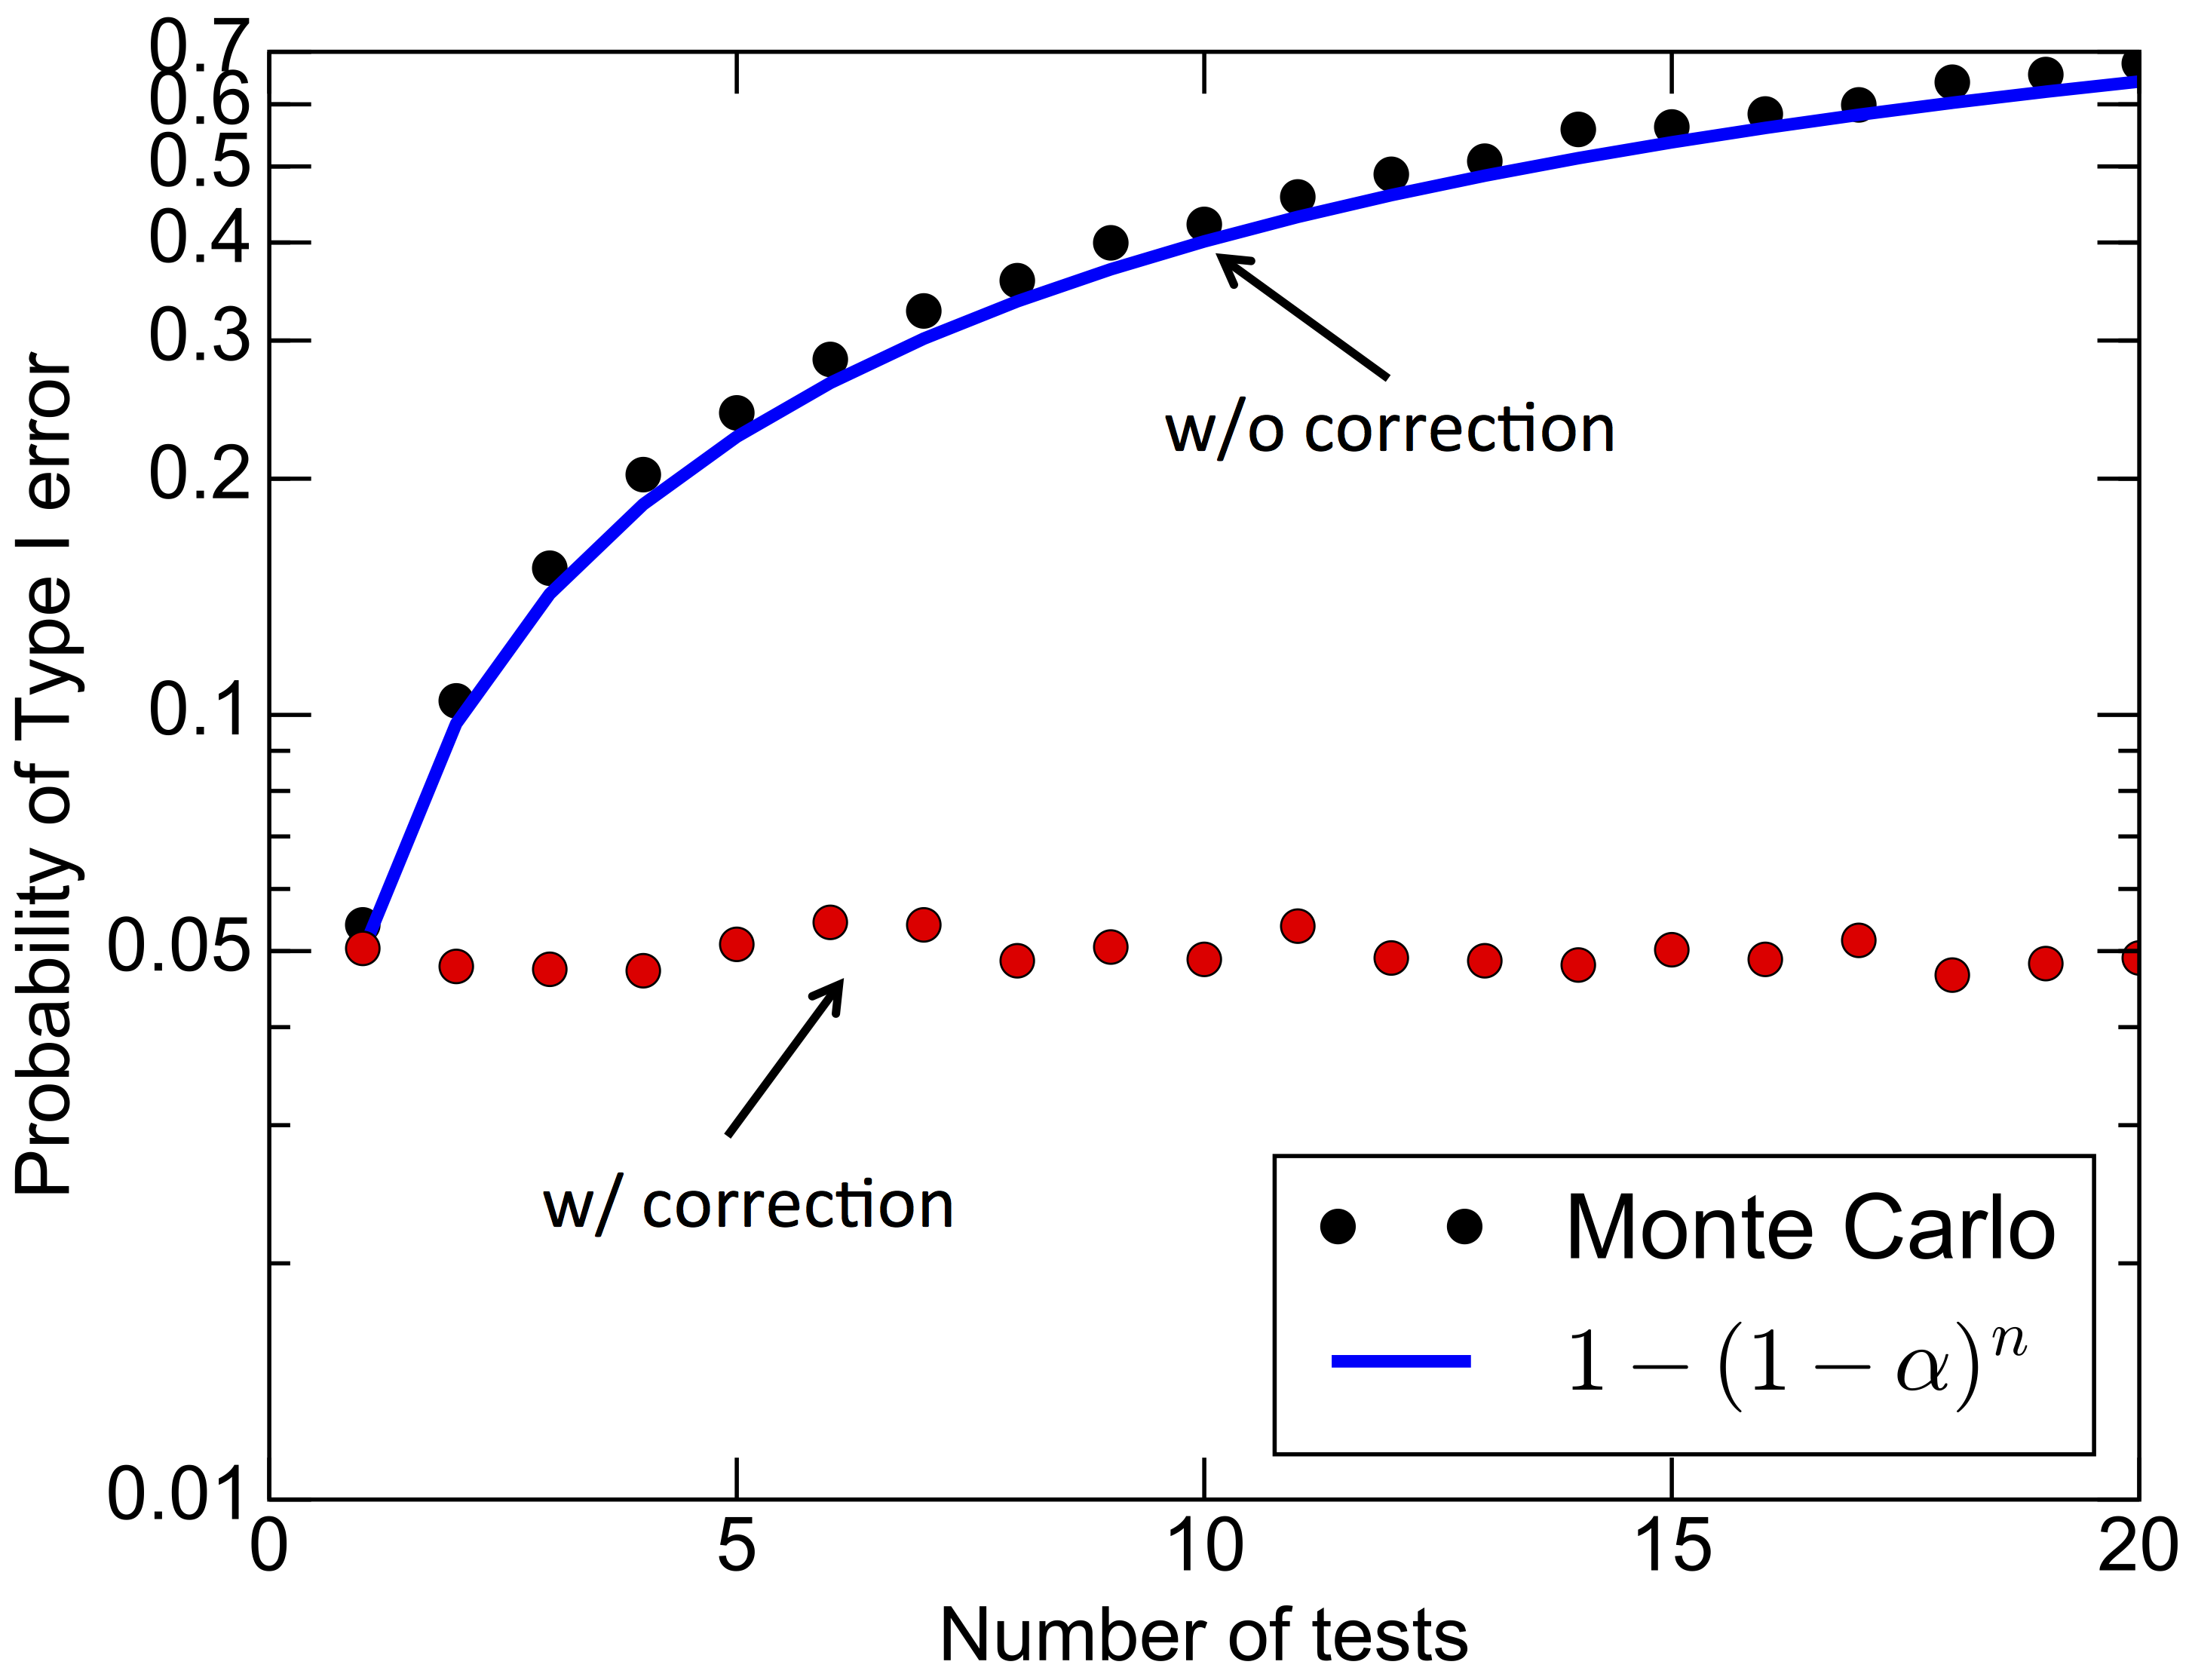
\includegraphics[width=\textwidth]{Lecture_Sources/Images/multiple_testing_loss_of_power.png}
\end{figure}
\end{frame}

\subsection{Контроль Family-wise ошибки}

% \begin{frame}{Как правильно тестировать несколько гипотез за раз}
% \begin{itemize}
%     \item $H_0$: верны все гипотезы $H_{0ti}$ 
%     \item $H_1$: верна хоть одна из гипотез $H_{1ti}$
% \end{itemize}

% \pause
% J-test: на доске
% \end{frame}

% \begin{frame}{Картинка}


% \end{frame}
% % Хорошо, а какая метрика прокрасилась?
% % А можно добавить

% \begin{frame}{Парные тесты с контроль Family-wise значиомсти}
%     квадратик
%     а как его обвести
% \end{frame}

\begin{frame}{Коррекция Бонферрони}
    Просто поделить уровень значимости на количество тестов
    $\alpha^\prime = \frac{\alpha}{m}$
    $$\text{FWER} \leq \sum_{i=1}^{m}P(testi|H_0))= m\alpha^\prime = \alpha$$ 
\end{frame}
% какие проблемы с тестом

\begin{frame}{Восходящая процедура Хольма}
    \begin{enumerate}
        \item Отсортировать увовни значимости тестов по возрастанию: $P_{(1)}$, $P_{(2)}$, ..., $P_{(m)}$
        \item Найти минимальный k такой, что $P_{(k)} > \frac{\alpha}{m+1-k}$
        \item отвергнуть все гипотезы с индексом $i < k$
    \end{enumerate}
\end{frame}
% почему она есть эта отсечка
% разобраться с формулой
% почему оно работает


\begin{frame}{Еще варианты}
    \begin{itemize}
        \item Коррекция Бонферрони
        \item Коррекция Сидака (альтернатива Бонферрони)
        \item Восходящая процедура Хольма
        \item Нисходящая процедура Сидака (альтернатива Хольму)
    \end{itemize}
\end{frame}


% это для умняшек
% IMAGE P VALUE VS
% LOSS OF POWER WITH CORRELATION
% boxes

% НО НАДО. ТАК ЯСНЕЕ